\documentclass[12pt]{article}
\usepackage{multicol}
\usepackage[utf8]{inputenc}
\usepackage[english]{babel}
\usepackage{graphicx}
\usepackage{amssymb}

\usepackage{geometry}
\geometry{top=10mm,left=10mm,right=10mm,bottom=17mm}

\usepackage{titlesec}
\titleformat{\section}{\Large\scshape\raggedright}{}{0em}{}[\titlerule]
\titlespacing{\section}{0pt}{3pt}{3pt}

\begin{document}

\section{Theory of Computation (Summary) \hfill Ayush Nath}
\bigskip
\large
\noindent \textbf{1. Automata and Languages}
\small
\begin{multicols}{2}
\noindent \textbf{1.1. Regular Languages}\\
\\
\textbf{Def.} A (deterministic) \textbf{finite automaton} is a 5-tuple $(Q, \Sigma, \delta, q_{o}, F),$ where
\begin{enumerate}
\itemsep-0.5em
\item $Q$ is a finite set called the \textbf{states},
\item $\Sigma$ is a finite set called the \textbf{alphabet},
\item $\delta: Q \times \Sigma \rightarrow Q$ is the \textbf{transition function},
\item $q_{o} \in Q$ is the \textbf{start state}, and
\item $F \subseteq Q$ is the set of \textbf{accepted/final states}
\end{enumerate}
\textbf{Def.} A language is called a \textbf{regular language} if some finite automaton recognizes it.\\
Ex. A language that has strings ending with 0; A language that has strings with substring 010.\\
\\
The class of regular languages is closed under the following operations:
\begin{enumerate}
\itemsep-0.5em
\item \textbf{Union}: $A \cup B = \lbrace x \mid x \in A or x \in B \rbrace.$
\item \textbf{Concatenation}: $A \circ B = \lbrace xy \mid x,y \in A,B \rbrace.$
\item \textbf{Star}: $A^{*} = \lbrace x_{1}, x_{2}, \dots, x_{k} \mid k \geq 0 $ and each $ x_{i} \in A \rbrace.$
\end{enumerate}
\textbf{Determinism}- When the machine is in a given state and reads the next input symbol, the next state is unique and already determined.\\
\textbf{Nondeterminism}- Several choices may exist for the next state at any point.\\
\\
\textbf{Def.} A \textbf{nondeterministic finite automaton} is the same 5-tuple, except
\begin{center}
$\delta: Q \times \Sigma_{\epsilon} \rightarrow P(Q)$
\end{center}
\textbf{Theorem.} Every NFA has an equivalent DFA.\\
\textbf{Corollary.} A language is regular if and only if some NFA recognizes it.\\
\\
\textbf{Def.} R is a \textbf{regular expression} if R is
\begin{enumerate}
\itemsep-0.5em
\item $a$ for some $a$ is the alphabet $\Sigma$,
\item $\varepsilon$,
\item $\phi$,
\item $(R_{1} \cup R_{2}),$ where $R_{1}$ and $R_{2}$ are regular expressions,
\item $(R_{1} \circ R_{2}),$ where $R_{1}$ and $R_{2}$ are regular expressions, or
\item $(R_{1}^{*})$, where $R_{1}$ is a regular expression.
\end{enumerate}
\textbf{Theorem.} A language is regular iff some regular expression describes it.\\
\textbf{Note.} Every regular language can be converted into an NFA.\\
\textbf{Note.} DFAs can be reduced to minimized DFAs.\\
\\
\textbf{Nonregular languages} are those that cannot be recognized by DFAs.\\
Ex. $\lbrace 0^{n}1^{n} | n \geq 0 \rbrace.$\\\\
\textbf{Theorem. Pumping Lemma} If $A$ is a regular language, then $\exists$ a number $p$ (the pumping length) where if any $s \in A$ s.t. $|a| \geq p,$ then $s$ can be divided into 3 pieces, $s=xyz$, s.t.
\begin{enumerate}
\itemsep-0.5em
\item for each $i \geq 0, xy^{i}z \in A,$
\item $|y| > 0,$ and
\item $|xy| \leq p.$
\end{enumerate}
Pumping Lemma can help differentiate between regular and nonregular languages.\\\\
\textbf{1.2. Context-free grammars}\\\\
\textbf{Def.} A CFG is a 4-tuple $(V, \Sigma, R, S),$ where
\begin{enumerate}
\itemsep-0.5em
\item $V$ is a finite set called the \textbf{variables},
\item $\Sigma$ is a finite set, disjoint from V , called the \textbf{terminals},
\item $R$ is a finite set of \textbf{rules}, with each rule being a variable and a string of variables and terminals, and
\item $S \in V$ is the \textbf{start variable}.
\end{enumerate}
A left hand derivation exists for every string $s \in L(CFG).$ The language of the grammar is $\lbrace w \in \Sigma^{*} | S \Rightarrow^{*} w \rbrace.$\\
Grammars can be unambiguous (i.e. each string has a unique LH derivation) or ambiguous (i.e. string has two or more LH derivations), or even inherently ambiguous.\\
\textbf{Note.} A context-free grammar is in Chomsky normal form if every rule is of the form
\begin{center}
$A \rightarrow BC$\\
$A \rightarrow a$\\
$S \rightarrow \varepsilon$
\end{center}
\textbf{Def.} A (nondeterministic) \textbf{pushdown automaton} is a 6-tuple $(Q, \Sigma, \varsigma, \delta, q_{0}, F),$ where
\begin{enumerate}
\item $Q$ is the set of \textbf{states},
\item $\Sigma$ is the \textbf{input alphabet},
\item $\varsigma$ is the \textbf{stack alphabet},
\item $\delta : Q \times \Sigma_{\varepsilon} \times \varsigma_{\varepsilon} \Rightarrow P(Q \times \varsigma_{\varepsilon})$ is the \textbf{transition function},
\item $q_{0} \in Q$ is the \textbf{start state}, and
\item $F \subseteq Q$ is the set of \textbf{accept states}.
\end{enumerate}
The stack gives the PDA a power of small storage.\\
\textbf{Theorem.}A language $A$ is a CFL iff $\exists$ a PDA $P$ s.t. $L(P) = A.$\\
Ex. $\lbrace 0^{i}1^{j}2^{k} | i \neq j or j \neq k, i,j,k \geq 0 \rbrace \in CFL.$\\\\
\textbf{Def.} A \textbf{deterministic PDA} is the same 5-tuple, except
\begin{center}
$\delta : Q \times \Sigma_{\varepsilon} \times \varsigma_{\varepsilon} \Rightarrow Q \times \varsigma_{\varepsilon} \cup \lbrace \phi \rbrace.$
\end{center}
s.t. $\forall q \in Q, a \in \Sigma, b \in \varsigma$ we have exactly one of the following to be non-empty:
\begin{center}
$\delta(q,a,b), \delta(q,a,\varepsilon), \delta(a,\varepsilon,b), \delta(\varepsilon,\varepsilon,\varepsilon)$
\end{center}
\textbf{Theorem.}A language $A$ is a DCFL iff $\exists$ a DPDA $D$ s.t. $L(D) = A.$\\
Ex. $\lbrace 0^{n}1^{n} | n \geq 0 \rbrace \in DCFL \setminus RL.$\\\\
\textbf{Note.} PDAs can either accept by final state or by emptying the stack.\\
\textbf{Note.} Every DPDA has an equivalent DPDA that always reads the entire input string.\\
\textbf{Note.} If $A = N(P)$ ,i.e. accepted by emptying the stack, then $A$ is prefix-free.\\\\
\textbf{Note.} CFLs are closed under union, intersections and complement.\\
\textbf{Note.} DCFLs are closed under complement.\\\\
\textbf{Def.} A \textbf{DCFG} is a CFG such that every valid string has a forced handle.
$\exists$ a similar pumping lemma for non-context-free languages where the string can be divided into five pieces instead, $s = uv^{i}xy^{i}z.$
\end{multicols}\bigskip
\large
\noindent\textbf{2. Computability Theory}
\small
\begin{multicols}{2}
\noindent\textbf{Def.} A \textbf{Turing Machine} is a 7-tuple $(Q, \Sigma, \tau, \delta, q_{o}$, $q_{a}, q_{r})$ where
\begin{enumerate}
\itemsep-0.5em
\item $Q$ is a finite set called the \textbf{states},
\item $\Sigma$ is a finite set called the \textbf{alphabet} and $B \not\in \Sigma$,
\item $\tau$ is the \textbf{tape alphabet} where $B \in \tau$ and $\Sigma \subseteq \tau$
\item $\delta: Q \times \tau \rightarrow Q \times \tau \times \big\{L,R\big\}$ is the \textbf{transition function},
\item $q_{o} \in Q$ is the \textbf{start state},
\item $q_{a} \in Q$ is the \textbf{accept state}, and
\item $q_{r} \in Q$ is the \textbf{reject state}.
\end{enumerate}
\textbf{Def.} The \textbf{configuration} of a machine is of the form $u_{1} u_{2} \dots u_{i-1} q u_{i} \dots u_{n}$ where $u_{j} \in \tau$. We say the machine is at state q and pointing to $u_{i}$.
\begin{enumerate}
\itemsep-0.5em
\item \textbf{Start:} $q_{0} u_{1} u_{2} \dots u_{n}$
\item \textbf{Accept:} $u_{1} u_{2} \dots u_{i-1} q_{a} u_{i} \dots u_{n}$.
\item \textbf{Reject:} $u_{1} u_{2} \dots u_{i-1} q_{r} u_{i} \dots u_{n}$.
\end{enumerate}
\textbf{Note.} During it's running, at any point if TM enters $q_{accept}$ or $q_{reject}$, it breaks and accepts or rejects respectively. This is known as accepting/rejecting by halting. If TM does not halt, a string is rejected by looping.\\\\
\textbf{Church-Turing Thesis.} Turing machines capture all algorithms, i.e. existence of an algorithm $\Rightarrow \exists$ a turing machine that can run it. \\\\
\textbf{Def.} A Language A is a \textbf{turing recognizable language} if $\exists$ a TM M such that $L(M) = A.$\\
\textbf{Def.} A Turing Machine M is a \textbf{Decider} if M halts for all input strings.\\
\textbf{Def.} A Language A is a \textbf{turing decidable language} if $\exists$ a decider M such that $L(M) = A.$\\
\textbf{Note.} Turing Decidable $\Rightarrow$ Turing Recognizable.\\
\textbf{Theorem.} All CFLs are decidable Turing Languages.\\\\
\textbf{Note.} $A_{TM}$ = $\big\{<M,w>$ $|$ M accepts w $\big\}$ is Turing recognizable but not Turing decidable, i.e., it is undecidable.
\\
\textbf{Def.} A language A is called \textbf{Co-Turing recognizable} if $A^{c}$ is Turing recognizable.
\\
\textbf{Theorem.} A language A is decidable $\Leftrightarrow$ A is Turing Recognizable and Co-Turing Recognizable.
\\
\textbf{Corollary.} $\overline{A}_{TM}$ is Turing Unrecognizable. 
\\\\
\textbf{Def.} For two languages A and B, \textbf{A reduces to B} means that $\exists$ a decider for B $\Rightarrow$ $\exists$ a decider for A. 
\\
\textbf{Note.} If A reduces to B and B is decidable $\Rightarrow$ A is decidable.
\\
\textbf{Note.} If A reduces to B and A is undecidable $\Rightarrow$ B is undecidable.
\\
\textbf{Ex.} $A_{HALT}$ = $\big\{<M,w>$ $|$ M halts on w $\big\}$. $A_{TM}$ reduces to $A_{HALT}$ and $A_{TM}$ is undecidable $\Rightarrow$ $A_{HALT}$ is undecidable.
\\\\
\textbf{Def.} A function f : $\Sigma^{*} \rightarrow \Sigma^{*}$ is a \textbf{computable function} if $\exists$ a TM M such that $\forall w \in \Sigma^{*}$, M halts with tape content as f(w). 
\\
\textbf{Def.} A language A is \textbf{Mapping Reducible} to language B (A $\leqslant_{M}$ B) if $\exists$ a computable function f : $\Sigma^{*} \rightarrow \Sigma^{*}$ such that $\forall w \in \Sigma^{*}$ and $w \in A$ $\Leftrightarrow$ $f(w) \in B$. 
\\
\textbf{Theorem.} A $\leqslant_{M}$ B and B is decidable $\Rightarrow$ A is decidable. 
\\
\textbf{Theorem.} A $\leqslant_{M}$ B and A is undecidable $\Rightarrow$ B is undecidable. 
\end{multicols}\pagebreak
\large
\noindent\textbf{3. Complexity Theory}
\small
\begin{multicols}{2}
\noindent\textbf{Def.} The \textbf{running time} of Turing Machine M is the function $f:N \Rightarrow N,$ where $f(n)$ is the max number of steps that M uses on any input of length n.
\\
\textbf{Note.} We say $f(n) = O(g(n))$ if positive integers $c$ and $n_{0}$ exist such that for every integer $n \geq n_{0}, f(n) \leq c \cdot g(n).$
\\
\textbf{Def.} The time complexity class, $TIME(t(n)),$ is the collection of all languages that are decidable by an $O(t(n))$ time Turing Machine.
\\
\textbf{Note.} All reasonable deterministic computational models are polynomially equivalent, i.e., any one of them can simulate another with only a polynomial increase in running time.
\\\\
\textbf{Def.} $P$ is the class of languages that are decidable in polynomial time on a deterministic single-tape Turing machine,
\begin{center}
$P = \bigcup\limits_{k}TIME(n^{k}).$
\end{center}
Ex. $PATH = \lbrace<G, s, t> | G$ is a directed graph that has a directed path from s to t$\rbrace; RELPRIME = \lbrace<x, y>| x$ and $y$ are relatively prime$\rbrace.$
\\
\textbf{Theorem.} Every CFL is a member of $P$.
\\\\
\textbf{Def.} A \textbf{verifier} for a language $A$ is an algorithm $V,$ where
\begin{center}
$A = \lbrace w | V$ accepts $<w, c>$ for some string $c \rbrace.$
\end{center}
Here, c is additional information, also called a \textbf{certificate.}\\\\
A \textbf{polynomial time verifier} runs in polynomial time in the length of w.\\
\textbf{Theorem.} $NP$ is the class of languages that have polynomial time verifiers.\\
Ex. $HAMPATH = \lbrace <G,s,t> \mid G$ is a directed graph with a Hamiltonian path from $s$ to $t \rbrace.$\\
\textbf{Theorem.} A language is in NP iff it is decided by some nondeterministic polynomial time Turing machine.\\
\textbf{Def.}
\begin{center}
$NTIME(t(n)) = \lbrace L \mid L$ is a language decided by an $O(t(n))$ time
nondeterministic Turing machine$\rbrace .$
\end{center}
\textbf{The} $\textbf{P}$ \textbf{vs.} $\textbf{NP}$ \textbf{Problem.}\\
$P$ = the class of languages for which membership can be decided quickly.\\
$NP$ = the class of languages for which membership can be verified quickly.
\begin{center}
$A \in P \Rightarrow A \in NP$ 
\end{center}
\textbf{Def.} Language $A$ is \textbf{polynomial time reducible} to language $B$ ($A \leqslant_{P} B$), if $\exists$ a polynomial time computable function $f: \Sigma^{*} \rightarrow \Sigma^{*}$ s.t.
\begin{center}
$w \in A iff f(w) \in B \forall w \in A$
\end{center}
\textbf{Note.} $B$ is called $NP-hard$ if $A \leqslant_{P} B \forall A \in NP.$\\
\textbf{Note.} $B$ is called $NP-complete$ if $B$ is $NP-hard$ and $B \in NP.$\\
Ex. $SAT, KSAT \in NP-complete.$
\end{multicols}
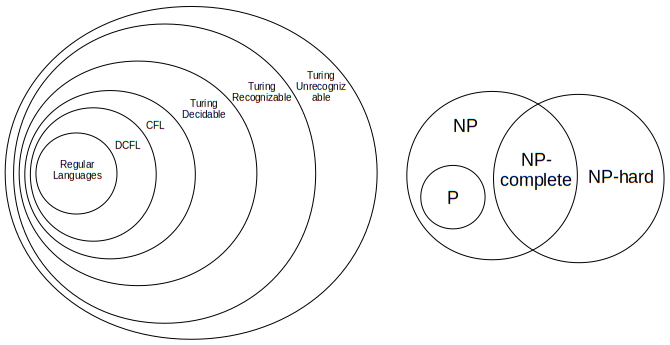
\includegraphics[scale=0.75]{6.png} 
\end{document}